\begin{figure}
    \centering
    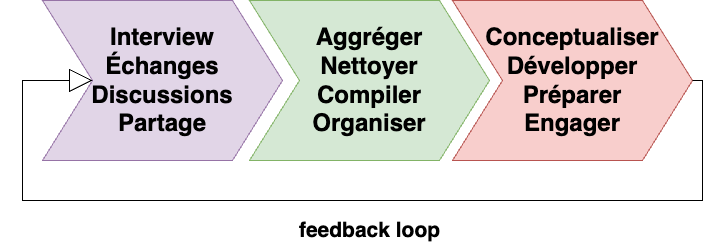
\includegraphics[width=0.75\linewidth]{images/Diagrams-Simplified framework chain Our approach.png}
    \caption{Notre approche simplifiée}
    \label{fig:simplified-approach}
\end{figure}

Notre travail s’inscrit dans le cadre de l’alliance universitaire européenne UNITA - Universitas Montium, composée de 12 institutions collaborant autour d’objectifs communs. Cette alliance constitue notre base d’expérimentation et illustre les défis auxquels les universités européennes de demain et plus généralement, les méta-organisations sont confrontées en matière d’évaluation d’impact sociétal.

Notre approche repose sur un cadre multi-axes conçu pour aider les méta-organisations, telles qu’UNITA, à évaluer leur impact en utilisant des méthodologies et outils orientés données (Figure~\ref{fig:simplified-approach}). Nous proposons une solution de stockage de données orientée impact, intégrant la collecte de preuves, l’analyse des indicateurs et des entretiens collaboratifs.

Les indicateurs d’outputs (résultats immédiats, comme le nombre de projets terminés) et d’outcomes (effets à moyen terme, comme l’augmentation de la collaboration entre membres) sont au cœur de cette démarche. Ces mesures permettent de suivre les progrès réalisés et de soutenir la prise de décision stratégique. 

Pour garantir la pertinence, notre méthode s’articule autour de trois étapes:
\begin{itemize}
    \item \textbf{Discussion} : Identifier les besoins spécifiques de chaque institution membre.
    \item \textbf{Évaluation} : Valider les indicateurs pour qu’ils soient fiables et adaptés aux objectifs stratégiques.
    \item \textbf{Construction} : Intégrer les données collectées dans un entrepôt structuré (DWH).
\end{itemize}

Les données intégrées dans le DWH, provenant de chaque institution, permettent de générer des rapports d’évaluation, d’identifier les tendances collaboratives et de suivre les progrès par rapport aux objectifs communs. Le nettoyage des données est une étape clé pour garantir la suppression des doublons, des erreurs et des incohérences issues des différentes équipes. Cela assure une intégration cohérente et une fiabilité accrue des analyses stratégiques.

Enfin, ce cadre vise non seulement à mesurer les résultats actuels, mais aussi à prédire l’impact futur des actions menées par l’alliance sur son environnement sociétal. Une précision accrue dans les données améliore directement la performance des modèles de prédiction, renforçant ainsi la capacité de l’alliance à anticiper les besoins et à adapter ses actions.
